\documentclass{standalone}
\usepackage[utf8]{vietnam}
\usepackage{graphicx}
\usepackage{booktabs}
\usepackage{amsmath}
\usepackage{textpos}
\usepackage{pgfplots}
\usepackage{tikz}
\usepackage{hyperref}
\usepackage{caption}
\usetikzlibrary{shapes.geometric, arrows}
\usetikzlibrary {datavisualization} 
\pgfplotsset{compat=1.18, width = 7cm}
\usetikzlibrary{patterns}
\usepackage{algorithm}
\usepackage{color}
\usepackage{algorithmic}
\usepackage{footmisc}
\usepackage{indentfirst} 
\usepackage{comment}
\begin{document}
    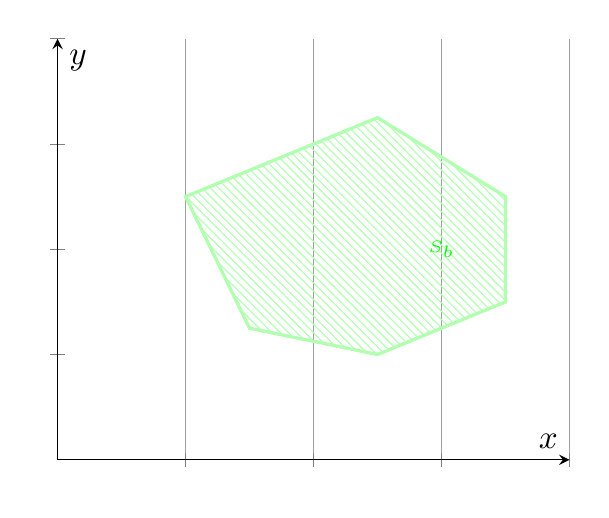
\begin{tikzpicture}[scale=1.2]
    \begin{axis}
        [
        xmin=0,xmax=80,
        ymin=0,ymax=80,
        xlabel={$x$},
        ylabel={$y$},
        grid style={line width=.1pt, draw=darkgray!50},
        major grid style={line width=.2pt,draw=darkgray!50},
        axis lines=middle,
        yticklabel=\empty,
        xticklabel=\empty,
        enlargelimits={abs=0},
        samples=100,
        xmajorgrids=true,
        domain = -20:20,
        ]
        \filldraw[green!30, pattern=north west lines, pattern color=green!30, line width=1pt] (30, 25) -- (50, 20) -- (70, 30) -- (70, 50) -- (50, 65) -- (20, 50) -- cycle;
        \node[green] at (60,40) {\tiny $S_b$};
    \end{axis}
    \end{tikzpicture}  
\end{document}